This multiple asset case is designed to test the computation of the individual asset loss curves, the portfolio loss exceedance curve, average asset losses, and the average portfolio loss, when the vulnerability models of different assets of the same taxonomy are treated as fully correlated. In OpenQuake, this can be specified in the job configuration file, by setting the value of the parameter `asset\_correlation' to one.

The list of assets and their taxonomies are shown in Table~\ref{tab:assets-tax1}. Table~\ref{tab:vf-ln-tax3-zcov} shows the mean loss ratios and corresponding coefficients of variation in the vulnerability function used in this test case.

Ground motion fields are generated for each of the ruptures generated in the 100,000 stochastic event sets as described in Case~6a and Case~6b. These ground motion fields are also used for the corresponding calculation in Julia.

Since the sampled loss ratios conditional on a given ground motion field for different assets of the same taxonomy are assumed to be fully correlated in this case, a single \emph{epsilon}, $\epsilon$,  is sampled from the standard normal distribution for each taxonomy. The parameters $m$ and $s$ from the vulnerability model are converted to the parameters $\mu$ and $\sigma$ of the corresponding normal distribution, and the sampled loss ratio is obtained simply as $\exp (\mu + \epsilon * \sigma)$.

The portfolio loss curve calculated using the implementation of the calculator in Julia is compared with that produced by OpenQuake in Figure~\ref{fig:lc-ebr-6c}. Only the aggregated results for the portfolio are shown here for brevity.

\begin{figure}[htbp]
\centering
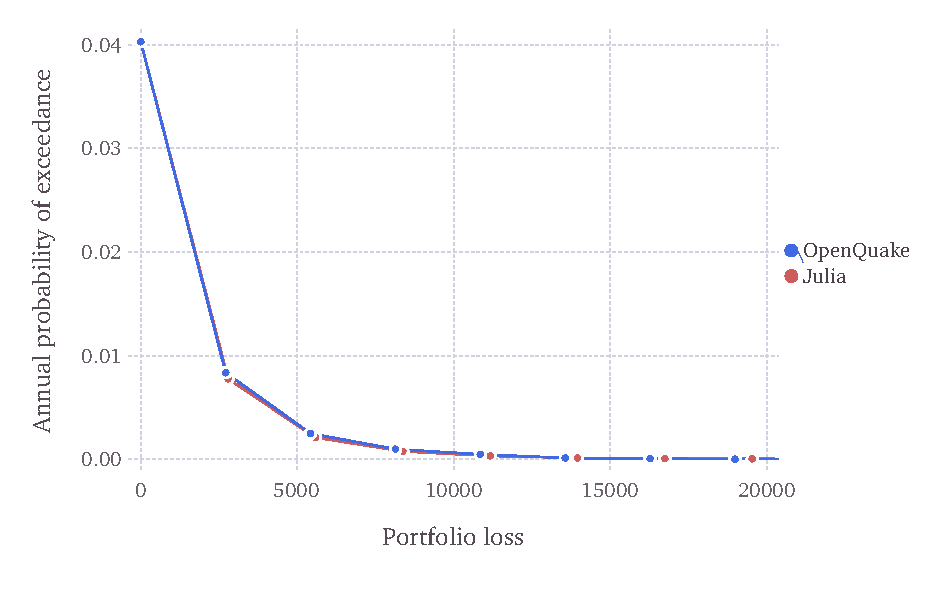
\includegraphics[width=12cm]{qareport/figures/fig-lc-ebr-6c}
\caption{Portfolio loss curve comparison for event based risk test case 6c}
\label{fig:lc-ebr-6c}
\end{figure}